\documentclass[10pt]{article}
\usepackage[margin=1in]{geometry}
\usepackage{amsmath,amssymb,amsthm}
\usepackage{graphicx}
\usepackage[hidelinks]{hyperref}
\usepackage{microtype}
\newtheorem{theorem}{Theorem}
\newtheorem{lemma}[theorem]{Lemma}
\newtheorem{corollary}[theorem]{Corollary}
\theoremstyle{definition}
\newtheorem{definition}[theorem]{Definition}
\theoremstyle{remark}
\newtheorem{remark}[theorem]{Remark}
\newtheorem{example}[theorem]{Example}
\usepackage{titlesec}
\titlespacing*{\section}{0pt}{10pt}{4pt}

\title{\bfseries Nomodynamics: The Mathematics of Self-Amending Law\\
\large A founding note}
\author{The Treeline Program}
\date{August 26, 2026}

\begin{document}
\maketitle
\vspace{-2em}
\begin{abstract}
\noindent Game theory formalized games with fixed rules; Conway's deletion of the
\emph{players} gave cellular automata and the Game of Life. The orthogonal
deletion---removing the \emph{fixity of the rules}---was never taken, although
rules that amend rules are humanity's oldest formal practice. We introduce a
minimal, parameter-free mathematical object native to that vacancy: a system
whose only substance is laws acting on laws. Its founding (``own-kind'')
semantics turns out to be exactly solvable, with short theorems that carry
immediate institutional readings: fully occupied codes are frozen
(\emph{gridlock}); stable codes are always fully blocked (\emph{dead letters});
and on the integer line \emph{the eldest law cannot be repealed}, which makes
free-moving law-packets impossible---and on circular codes, which have no eldest
law, what looks like a moving packet turns out to be a barber pole. The solvable sector exhibits a small
charismatic fauna (colonizers, sunset clauses, welds, refraction, apparent
rotations, and an aperiodic avalanche machine locked to powers of two). Letting
laws amend \emph{other} laws then settles what motion costs: a tropical
monovariant shows that a constitution in which every law amends a single
kind---anyone's kind---is motionless in every dimension, window and resolution,
while two targets suffice, and the smallest traveller is one placed law. The
same generalization splits the stability theorem by resolution convention and
produces \emph{balanced constitutions}: codes perpetually active and perfectly
unchanging. Dropping instead the tacit assumption that laws are permanent
inverts the founding theorem---the very first specimen becomes a glider, and a
packet's speed is set by how long a provision survives unrenewed. Finally the
system computes: a provision that repeals itself every step is a register, a
constitution in the resulting normal form is a synchronous AND-NOT network,
Rule~110 runs inside a $24$-kind constitution, and every Turing machine compiles
into a finite code---so the field is computation-universal, with halting
undecidable, while every one of its provisions stands still.
\end{abstract}

\section{The vacancy}
Three observations, from a systematic survey of how new mathematical ontologies
have historically been found, converge on one empty cell.
(\emph{i})~The deletion grid: von Neumann--Morgenstern formalized $2$-player
fixed-rule games; puzzles are the $1$-player case; Conway's
``$0$-player games'' are cellular automata. Along the orthogonal axis---rule
fixity---no elementary mathematics exists.
(\emph{ii})~The reduction shadow: computability theory's founding reduction,
``without loss of generality the program is fixed,'' is valid for
\emph{what can be computed} (universality lets a fixed machine simulate a
self-modifying one) but silently discards the \emph{behavioral} questions: what
do small self-amending systems actually do? Nobody looked, because the
reduction said one need not.
(\emph{iii})~The practiced verb: constitutions and statutes---self-amending by
essence---are the oldest running formal systems, yet ``amend'' was never
objectified the way Church and Turing objectified ``compute.'' The fragments
that exist (von~Neumann's rule-carrying constructor cells; Suber's game
\emph{Nomic}, 1982; self-modifying Petri nets, 1978; algorithmic chemistry)
never produced a minimal canonical object, a census, or a theorem.

\section{The object}

\subsection*{2.1\quad The founding system}
Fix the finite set $K_0=\{-1,0,1\}^3$; its elements are called \emph{kinds}.
For a kind $k=(a,b,c)$ the three integers are its \emph{precedent}, its
\emph{exception} and its \emph{target} offset. A \emph{placed law} is a pair
$(i,k)\in\mathbb{Z}\times K_0$; a \emph{code} is a finite set
$S\subseteq\mathbb{Z}\times K_0$ of placed laws; $\mathcal{S}$ denotes the set
of codes. Write
\[
  \operatorname{occ}(S)=\{\,i\in\mathbb{Z}\ :\ (i,k)\in S\ \text{for some }k\in K_0\,\}
\]
for the set of \emph{occupied} positions.

\begin{definition}[activity]
A placed law $(i,k)\in S$ with $k=(a,b,c)$ is \emph{active in} $S$ if
$i+a\in\operatorname{occ}(S)$ and $i+b\notin\operatorname{occ}(S)$. Let $A(S)$
denote the set of placed laws active in $S$.
\end{definition}

\begin{definition}[nomic chain]\label{def:chain}
Every $(i,k)\in A(S)$ with $k=(a,b,c)$ \emph{emits a toggle} of the placed law
$(i+c,k)$. Let $T(S)$ be the multiset of all emitted toggles and let
$T_{\mathrm{odd}}(S)\subseteq\mathbb{Z}\times K_0$ be the set of placed laws
occurring in $T(S)$ an odd number of times. The successor of $S$ is
\[
  \Phi(S)\;=\;S\ \triangle\ T_{\mathrm{odd}}(S)
  \qquad(\triangle=\text{symmetric difference}),
\]
and the \emph{nomic chain} is the discrete dynamical system
$(\mathcal{S},\Phi)$, iterated synchronously.
\end{definition}

\noindent In words: a law acts when the position named by its precedent offset
is occupied and the position named by its exception offset is empty; its action
is to insert a law of its own kind at the position named by its target offset if
none stands there, and to delete it if one does. $\Phi$ is well defined because
$S$ is finite, hence so are $A(S)$ and $T(S)$.

\begin{example}
Let $k=(0,1,1)$ and $S_0=\{(0,k)\}$, a single law at the origin. Then
$\operatorname{occ}(S_0)=\{0\}$; the law is active, since $0+0\in
\operatorname{occ}(S_0)$ and $0+1\notin\operatorname{occ}(S_0)$; it emits a
toggle of $(1,k)$, which lies outside $S_0$, so
$S_1=\Phi(S_0)=\{(0,k),(1,k)\}$. At the next step the law at $0$ is inactive
($0+1$ is now occupied) while the law at $1$ is active, so
$S_2=\{(0,k),(1,k),(2,k)\}$, and inductively $S_n=\{(0,k),\dots,(n,k)\}$: the
kind $(0,1,1)$ fills the line rightwards at one position per step, only ever
acting at its own frontmost copy. Under the lifetime variant with $\tau=1$ the
same computation gives $S_n=\{(n,k)\}$ instead --- the single law walks
(\S7).
\end{example}

\subsection*{2.2\quad The general object}
The later chapters each replace exactly one clause. A \emph{constitution}
consists of a finite set $K$ together with, for every $k\in K$: offsets
$a_k,b_k,c_k\in\{-w,\dots,w\}^d$, a \emph{target set} $T_k\subseteq K$, and a
pair of \emph{citations} $g_k,h_k\in K\cup\{\ast\}$. Codes are now finite
subsets of $\mathbb{Z}^d\times K$. For $x\in K\cup\{\ast\}$ and a position $p$
write
\[
  S\models x@p
  \quad:\iff\quad
  \begin{cases} p\in\operatorname{occ}(S) & x=\ast,\\[2pt]
                (p,x)\in S & x\in K,\end{cases}
\]
so $\ast$ reads \emph{some law stands here} and $x\in K$ reads \emph{that
particular kind stands here}. Then
\[
  (i,k)\in A(S)\iff S\models g_k@(i+a_k)\ \text{ and }\ S\not\models h_k@(i+b_k),
\]
every active $(i,k)$ emits a toggle of $(i+c_k,t)$ for each $t\in T_k$, and
$\Phi$ is as in Definition~\ref{def:chain}. The founding system is the case $d=w=1$, $K=K_0$,
$T_k=\{k\}$ and $g_k=h_k=\ast$; chapter two varies $T_k$, chapter three varies
$(g_k,h_k)$.

\subsection*{2.3\quad Variants}
Each of the following substitutes for one clause and leaves the rest intact.
\begin{itemize}\itemsep1pt \parskip0pt
\item \emph{Rings.} Replace $\mathbb{Z}^d$ by $(\mathbb{Z}/m)^d$.
\item \emph{Resolution.} Parity, as above, or \emph{OR}:
 $\Phi_{\vee}(S)=S\,\triangle\,\operatorname{supp}T(S)$, where a toggle lands if
 it is emitted at all. The two coincide whenever no placed law receives two
 toggles in the same step.
\item \emph{Supersession.} An active law enacts its own kind at $i+c_k$ if that
 position is empty, and otherwise deletes every law standing there.
\item \emph{Lifetime $\tau\in\{1,2,\dots\}\cup\{\infty\}$.} Effects are
 \emph{enactments} rather than toggles: an active law inserts $(i+c_k,t)$ for
 each $t\in T_k$, and a placed law survives a step only if it is enacted now or
 has been enacted within the previous $\tau-1$ steps. Chapters one to three are
 the toggle semantics; chapter four is $\tau<\infty$.
\end{itemize}

\noindent There is no board, no background and no external rule table: the only
data is which laws stand where, and the rule a law obeys is the law itself. The
founding system in particular has no parameters --- $K_0$ has $27$ elements and
that is the entire specification. All claims below were pre-registered as
predictions or risks before the first simulation, then settled by censuses with
machine-checked certificates ($\sim$15.3 million certified runs for the no-go
results; complete enumerations where stated); \texttt{verify.py} in the archive
re-derives every named claim from the definitions above.

\section{First theorems: the solvable sector}
\begin{theorem}[Gridlock]
In a fully occupied region every law's vacancy guard fails; a solid code is
frozen. All dynamics is surface dynamics.
\end{theorem}
\begin{lemma}[Single Author]
The only law that can ever flip kind $k=(a,b,c)$ at position $j$ is the
kind-$k$ law at $j-c$. Hence parity and idempotent (``OR'') resolution
coincide identically, in every dimension, and per-kind dynamics is
occupancy-modulated linear algebra over $\mathbb{F}_2$.
\end{lemma}
\begin{theorem}[Dead Letter]
A code is a fixed point iff every law in it is blocked. In particular
\emph{balanced constitutions}---codes in perpetual self-cancelling
activity---do not exist: stability is always gridlock.
\end{theorem}
\begin{theorem}[Anchor]
On $\mathbb{Z}$ (any window, any dimension, any guard predicate, either
resolution semantics), own-kind toggles of kind $t$ land only at $t$'s own
offset $c_t$; consequently the extremal law on the trailing side of a finite
code is never targeted: \emph{the eldest law cannot be repealed}. No finite
code satisfies $\Phi^p(S)=\sigma^d(S)$ with $d\neq0$: free gliders are
impossible.
\end{theorem}
\begin{corollary}[Ring rotors---and what they are not]
On $\mathbb{Z}/m$ there is no eldest law, and codes appear that coincide with
their own rotation: three laws of the single kind $(0,1,-1)$ at cells
$\{1,2,5\}$ of $\mathbb{Z}/6$ satisfy $\Phi(S)=\mathrm{rot}_3(S)$
(Fig.~\ref{fig:rotor}), and the family runs over every even $m\ge6$---the block
word forces $m=2\gamma+4$ with hop $m/2$, so the evenness is a theorem, not a
survey. \emph{But this is not transport.} Window-1 laws move information at most
one cell per step, so a rotation by $m/2$ in a single step cannot be carrying
anything: exactly two cells change---a repeal at $1$, an enactment at $4$---and
the new state merely happens to equal the old one rotated (the seed has no
rotational symmetry, so $3$ is the only rotation relating them). Every own-kind
ring rotor fails this light-cone test, and releasing $19{,}074$ of them onto
$\mathbb{Z}$ yields zero gliders. \emph{Own-kind nomodynamics contains no
transport at all: not on the line, and not on the circle. What a ring supplies
is apparent rotation---a barber pole.}
\end{corollary}
\begin{remark}
The lemma explains the observed clockwork: every exact cycle found across
$\sim$140{,}000 seeds has period a power of two, and single-kind ring codes
(the ``Sunset Parliament'') attain exact maximal periods $15$, $63$, $341$ at
resonant circumferences $m\equiv2\ (\mathrm{mod}\ 4)$---orders of
$\mathbb{F}_2$-polynomials governing constitutional cycles.
\end{remark}

\section{Fauna of the solvable sector}
\begin{figure}[t]
\centering
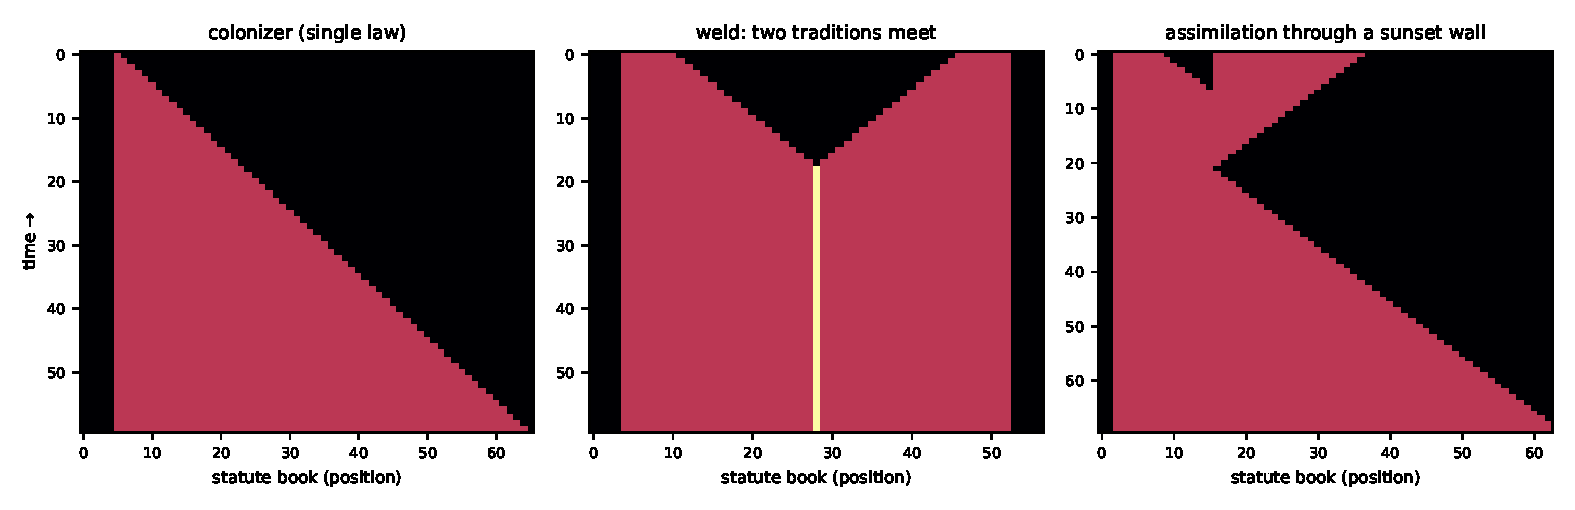
\includegraphics[width=\textwidth]{fig1_spacetime.pdf}
\caption{Window-1 nomic chains (time downward). Left: the \emph{colonizer}
$(0,1,1)$---``while I stand and my right is vacant, enact my kind to the
right''---only its frontmost copy is ever active. Middle: two traditions
meet and \emph{weld} into frozen code with a double-law seam. Right: a
colonizer meets a self-eroding \emph{sunset wall}. The wall repeals itself from
its far end while the front stands blocked; the front then fills the vacated
ground, so a wall of length $L$ is cleared at time exactly $\max(2L,\,x_0+L)$
--- the ``refraction index~2'' is those two speed-1 processes in sequence. The
colonizer never converts the wall: it waits for the old code to sunset and
takes the vacancy.}
\label{fig:spacetime}
\end{figure}
\begin{figure}[t]
\centering
\begin{minipage}{0.30\textwidth}
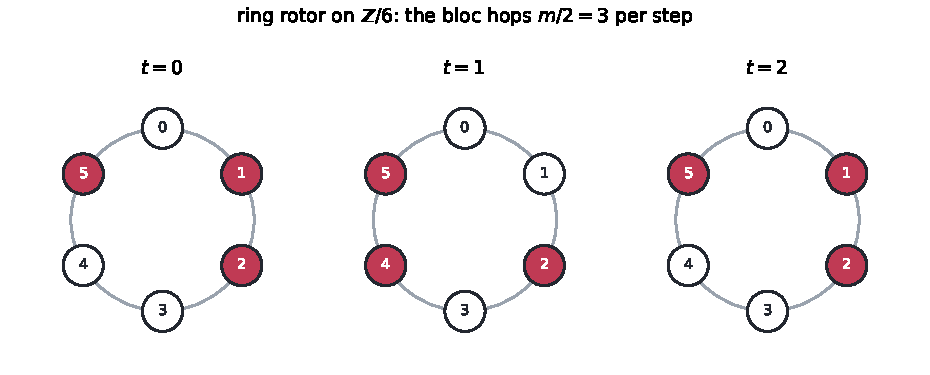
\includegraphics[width=\textwidth]{fig2_rotor.pdf}
\end{minipage}\hfill
\begin{minipage}{0.66\textwidth}
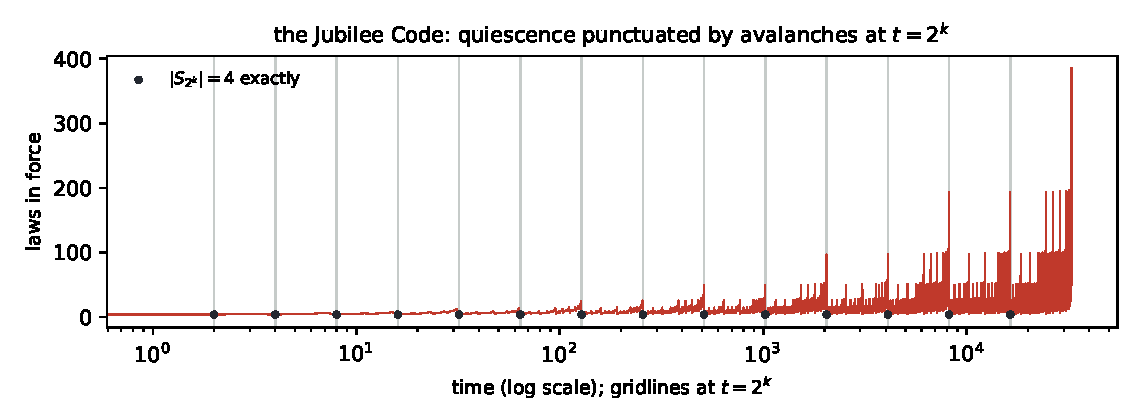
\includegraphics[width=\textwidth]{fig3_jubilee.pdf}
\end{minipage}
\caption{Left (\ref{fig:rotor}): the $\mathbb{Z}/6$ ring code that coincides with its own rotation by three---an apparent rotation, not transport. Right: the
\emph{Jubilee Code}, a $\sim$26-law two-dimensional machine, aperiodic through
300{,}000 fully-hashed steps and quiescent except at $t=2^k-1$, when the
counter fills and the whole code ignites; at $t=2^k$ itself exactly four laws
stand, every time (16/16, complete through $t<2^{17}$), and the crest height
doubles every second power of two. A binary counter native to law-space, and an
attractor: $791$ of $60{,}000$ random seeds converge to its family.}
\label{fig:rotor}
\end{figure}
The one-dimensional chain is a calculus of fronts (Fig.~\ref{fig:spacetime}):
\emph{colonizers} (2 of the 27 kinds) fill the line at speed 1;
the \emph{sunset clause} $(0,-1,1)$ forever enacts a subordinate its own
presence then blocks (period 2); \emph{sunset codes} dissolve from their
newest end; colliding fronts \emph{weld}; porous codes support one-way
\emph{conversion waves} (speed $2/3$); walls facing a front sort into opaque
(19/27), pulsing (3/27), and effectively transparent (5/27) classes.
In two dimensions a \emph{ray-confinement theorem} pins each kind to one axis
ray (quadrants never fill), and the fauna adds 239 certified half-turn
\emph{pinwheel rotors}, Pascal-column growers with
$|S_t| = 2^{\mathrm{popcount}(t)}$, and the Jubilee Code (Fig.~\ref{fig:rotor},
right). Finite rings admit an exact fixed-point count (transfer matrix,
brute-force verified), a predecessor algebra with Garden-of-Eden fraction
peaking $\approx33\%$ at mid-density, and a unique minimal taut architecture
(the two-law \emph{mutual-veto} pair).

\section{Cross-amendment: what motion costs}
Own-kind amendment is the tame simplification; real statutes amend other
statutes. Generalize minimally: a \emph{constitution} is a finite kind set $K$,
each $k\in K$ carrying a rule $(a_k,b_k,c_k)$ and a \emph{target set}
$T_k\subseteq K$; an active law of kind $k$ at $i$ toggles every kind of $T_k$
at $i+c_k$. Own-kind is $T_k=\{k\}$. Nothing external is added: out-degree~1
makes the amendment digraph a functional graph, so a kind is a pointed finite
graph with a triple at each node---\emph{``I am $(a,b,c)$, and I amend the law
that is $(a',b',c')$ and amends\dots''}---and own-kind laws are exactly the
self-loops. The law is still the only substance.

The expectation was that cross-kind targeting is the escape from the Anchor
Theorem. It is not.
\begin{theorem}[Out-Degree Law]
If, restricted to the kinds a pattern uses, every law amends \emph{at most one}
kind, no free glider exists---any offsets, any window, any dimension, parity or
OR. This contains the Anchor Theorem (self-loops), reciprocal amendment, and
every permutation constitution of every cycle length.
\end{theorem}
The proof is a tropical monovariant: with weights $w$ satisfying
$w_k-c_k\le w_{t(k)}$, the quantity $\Psi=\min_t(\alpha_t+w_t)$ over the kinds'
trailing edges can rise only through a tight cycle of weight~$0$. The same
argument bounds speed.
\begin{theorem}[Tropical Speed Law]
For a glider of period $p$ and displacement $d$,
$p\min(\lambda_{\min},0)\le d\le p\max(\lambda_{\max},0)$, where
$\lambda_{\min},\lambda_{\max}$ are the extreme cycle means of the amendment
digraph (edge $k\to m$ of weight $c_k$ for each $m\in T_k$). If every cycle has
weight zero, or the digraph is acyclic, nothing moves.
\end{theorem}
\begin{theorem}[Supersession no-go]
State-dependent \emph{supersession} targeting---enact your own kind on empty
ground, clear the whole cell if occupied---admits no free glider in any
dimension: its creation channel is still own-kind, so every present kind must
push forward, and then nothing can clear the rearmost cell.
\end{theorem}
\begin{figure}[t]
\centering
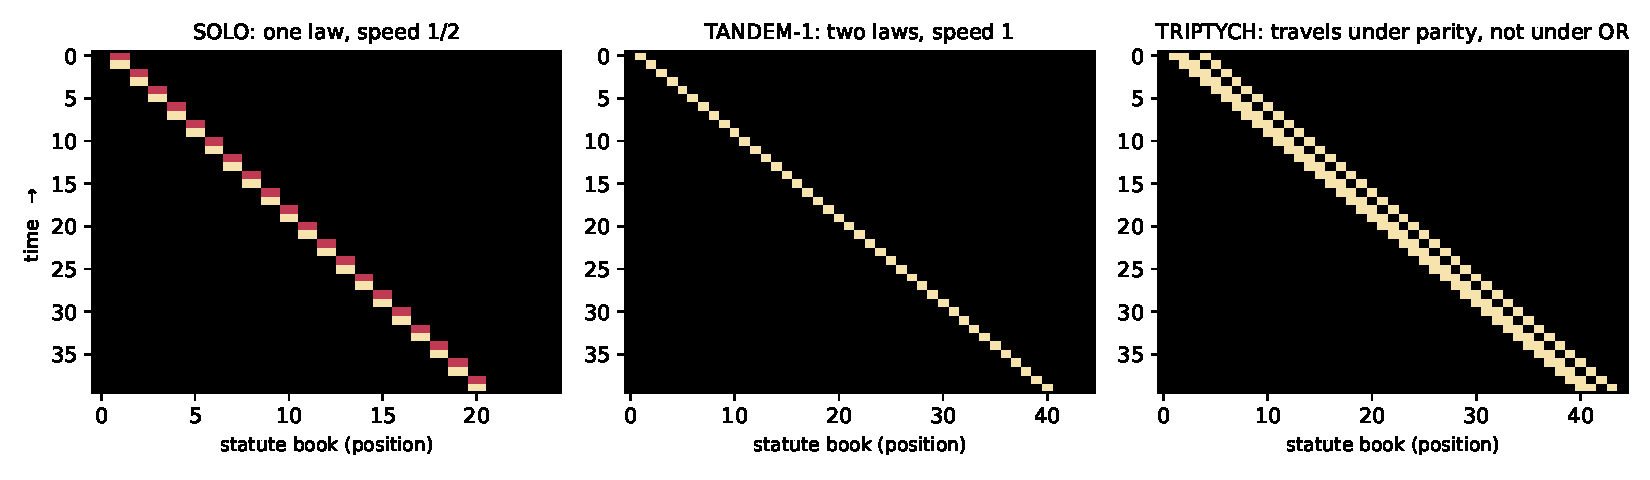
\includegraphics[width=\textwidth]{fig4_gliders.pdf}
\caption{The first free gliders of nomodynamics (time downward).
\emph{SOLO}: one placed law travelling forever at speed $\frac12$ under a
fully-cross constitution. \emph{TANDEM-1}: two laws in a \emph{single} cell,
period~1, speed~1---the maximum; it lifts to $\mathbb{Z}^2$ at any velocity,
knight moves included, and revolves on every ring $m\ge3$, where own-kind
rotors need even $m\ge6$. \emph{TRIPTYCH}: a glider under parity that under OR
does not travel at all but detonates into a lattice growing by three laws per
step.}
\label{fig:gliders}
\end{figure}
\emph{The threshold is exact}: out-degree $2$ suffices and the specimens are
tiny (Fig.~\ref{fig:gliders}). The cleanest evidence is a controlled
experiment---three semantics sharing their guards, their offsets and their
destruction rule exactly and differing only in the out-degree of the
\emph{creation} channel---giving $0$ gliders in $1{,}119{,}744$ complete
classifications at out-degree~$1$ and $3{,}424$ certified gliders in
$279{,}936$ at out-degree~$2$. So
\emph{cross-amendment was never the obstruction: narrowness was.} A law that
amends one provision, even somebody else's, cannot move; a law that amends two
can. Entrenchment, in chapter one a consequence of linear order, is equally a
consequence of legislative narrowness.

\begin{figure}[t]
\centering
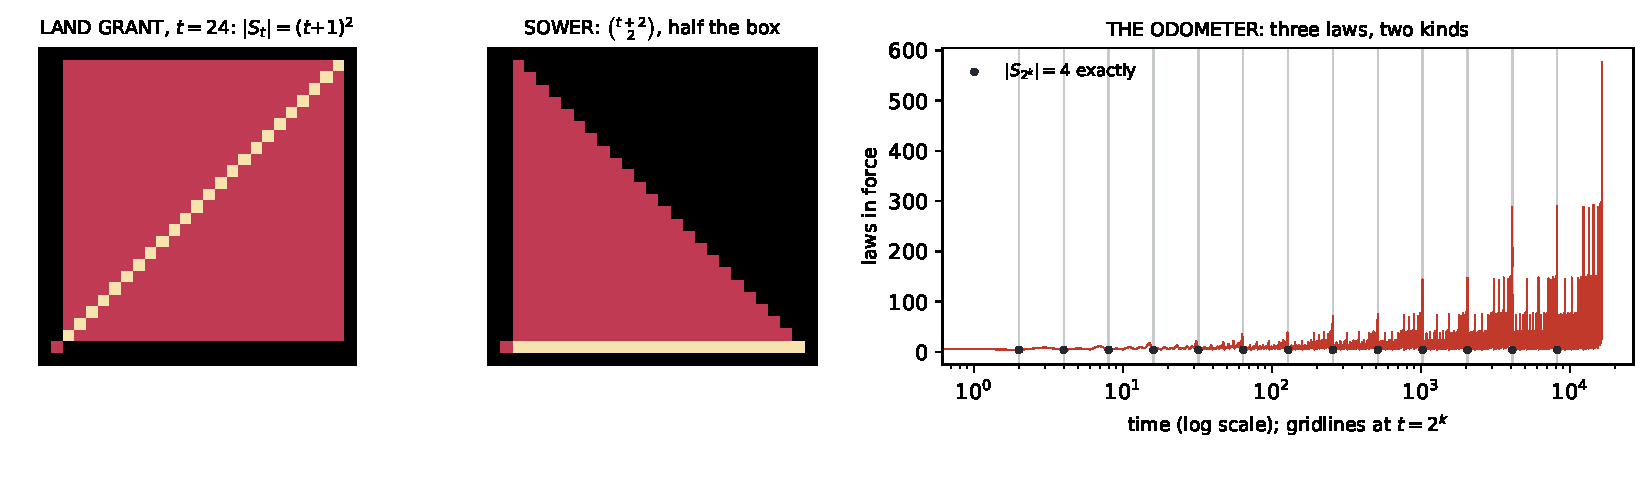
\includegraphics[width=\textwidth]{fig5_plane.pdf}
\caption{Two dimensions. Left: \emph{Land Grant}---one law with two targets,
and $|S_t|=(t+1)^2$ exactly, a solid growing square: the plane fills, which
own-kind ray confinement forbids. Middle: \emph{Sower}, two laws, exactly half
the box. Right: \emph{the Odometer}, three laws of two kinds, a second binary
counter---quiescent, avalanching at $2^k-1$, and standing at exactly four laws
at every $t=2^k$ (checked to $t=2^{20}$), with reach growing like
$(\log t)^2$: bounded population, unbounded memory, never repeating.}
\label{fig:plane}
\end{figure}
The same degree condition governs \emph{growth}. Own-kind two-dimensional
growth is pinned to axis rays ($\alpha\le1$, a theorem of chapter one); the
generalisation is exact and cheap: out-degree~$1$ forces
$|S_t|\le|S_0|(t+1)$---hence $\alpha\le1$ in every dimension, under parity, OR
and supersession alike---while out-degree~$2$ attains $\alpha=2$ from a single
placed law (Fig.~\ref{fig:plane}). Ray confinement was never a fact about two
dimensions; it was a fact about narrow laws. The degrees of the amendment
digraph turn out to govern the whole zoo: out-degree $\le1$ forbids motion and
caps growth; out-degree~$\ge2$ buys gliders and area; a kind of \emph{in-degree
zero}---a provision nobody can amend---is a pump, and yields guns and rakes,
on $\mathbb{Z}$ as readily as on $\mathbb{Z}^2$. \emph{An entrenched clause is
a gun.}

Cross-amendment also explains chapter one's clockwork rather than merely
extending it. The frozen-occupancy step operator of an $L$-cycle permutation
constitution lives in $\mathbb{F}_2[y]/(y^L-1)$, \emph{which is local exactly
when $L$ is a power of two}. So ``all periods are powers of two'' was never a
fact about own-kind amendment; it was a fact about \emph{cycle length one}---and
$1$ is a power of two. An odd factor $L'\mid L$ contributes $\mathbb{F}_{2^d}$
factors with $d=\mathrm{ord}_{L'}(2)$, and the odd periods appear at once:
predicted and measured at every $L\le7$ ($L=3\to3$, $L=5\to15$, $L=7\to7$), and
on the three-cell ring a five-cycle constitution realises every odd period
through $15$ from two laws. A new resonance family appears at powers of three
where own-kind gave Mersenne numbers. On rings, cross-amendment also lowers the
minimal rotor circumference from six to four, reaches odd rings for the first
time (always with $r\equiv\pm m/3$), and produces an object with no own-kind
analogue: a \emph{doctrinal rotor} whose occupied cells never change while the
\emph{kinds} circulate through them and return after three steps---a code frozen
on its face whose doctrine rotates underneath.

Multi-authorship also revives the resolution axis that the Single-Author Lemma
had made vacuous, and it kills the Dead Letter Theorem in exactly one
convention.
\begin{theorem}[Balance]
Under parity, two active laws whose enactments cancel leave a code fixed
forever while remaining alive---a \emph{balanced constitution}; the minimal
witness is two placed laws. Under OR no such code exists at any size: a fixed
point still requires every law blocked, and Dead Letter survives verbatim.
\end{theorem}
\noindent A constitution can be perpetually active and perfectly unchanging---
but only where simultaneous contradictory amendments annul one another instead
of both taking effect. Balance is governed by the \emph{other} degree: a
provision with two authors. It is not a curiosity of small codes---balanced
codes of unbounded size exist with \emph{every} law active at every step, their
exact count satisfies $a(s)=4a(s-1)-2a(s-2)$, and $70\%$ of the balanced
verdicts in a complete $143$-million-run census are reached rather than seeded.

Finally, the Anchor Theorem itself has a deeper reading than ``own-kind
amendment forbids motion''. A sweep of the semantics the referent
suggests---entrenchment clauses, quorum guards, later-law-wins,
sunset-by-default---finds that all but one leave the confinement theorems
untouched (they are guard-free), while \emph{sunset-by-default}, where a law
lapses unless re-enacted, admits free gliders on $\mathbb{Z}$ with plain
own-kind targeting: $11$--$15\%$ of a complete $139{,}968$-code box, at speeds
$1,\ \frac23,\ \frac12,\ \frac13,\ \frac14,\ \frac16$. So there are exactly two
ways known to make a statute book move:
\begin{center}
\emph{legislate broadly (out-degree $\ge2$), or let provisions expire on their
own.}
\end{center}
\noindent What forbids motion on the line is \textbf{permanence}, not own-kind
targeting---the Anchor Theorem's real content.

\section{Impermanence: motion is a consequence of mortality}
Every sector so far assumes a law stands until something repeals it. That
assumption is load-bearing and nobody had weighed it. Drop it:
take the lifetime $\tau$ of \S2.3 to be finite, so that effects are enactments
and a placed law survives only while it keeps being re-enacted. To repeal is
then simply to stop re-enacting, and $\tau=1$ is the pure case: what stands next
is exactly what is enacted now.
\begin{figure}[t]
\centering
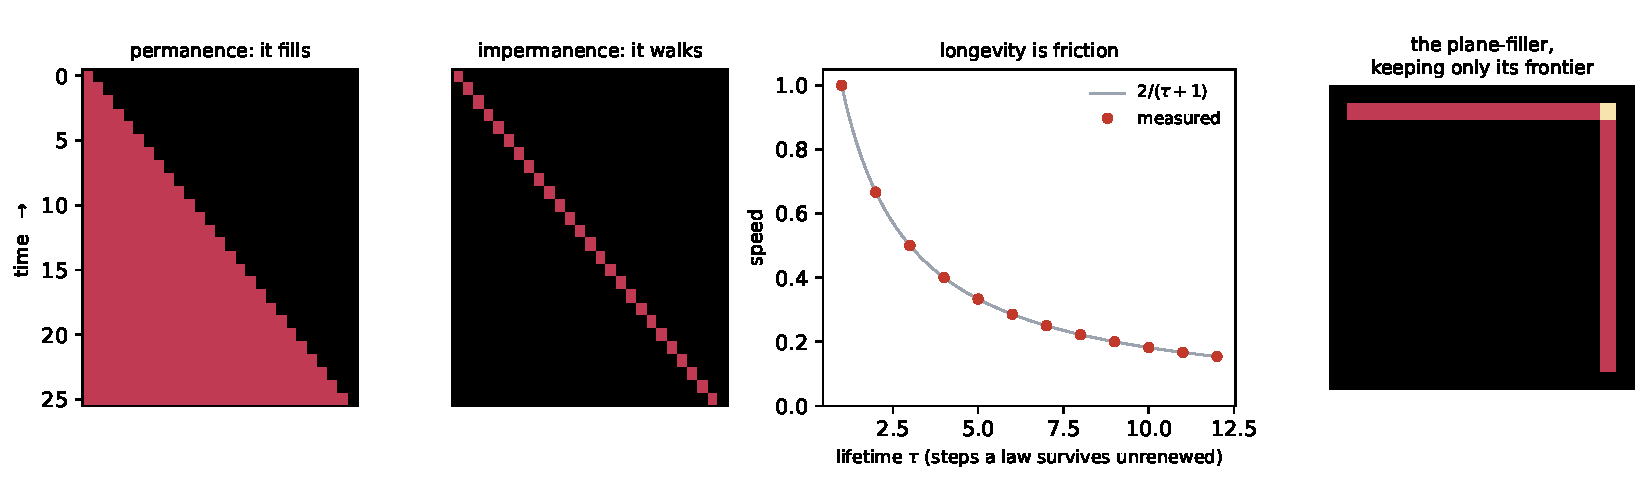
\includegraphics[width=\textwidth]{fig6_impermanence.pdf}
\caption{Impermanence. The colonizer $(0,1,1)$---the same law, the same guard,
the same target---\emph{fills} the line when provisions are permanent and
\emph{walks} when they lapse. Third panel: one code, one seed, and the lifetime
$\tau$ as a dial; the packet always moves two cells but must wait for its own
tail to lapse, so its speed is exactly $2/(\tau+1)$ (measured points, certified
$\tau\le12$). Right: \emph{Land Grant}, whose population is $(t+1)^2$ under
permanence, keeps only the two advancing edges of that square.}
\label{fig:sunset}
\end{figure}
\begin{theorem}[Lone Survivor]
Under $\tau=1$ a single placed law of kind $(a,b,c)$ survives its first step iff
$a=0$ and $b\neq0$---its precedent is itself and its exception is elsewhere. It
then translates by $c$ forever: it \emph{walks} if $c\neq0$ and renews itself in
place if $c=0$. The other $21$ of the $27$ kinds vanish in one step.
\end{theorem}
So chapter one's very first specimen becomes a glider (Fig.~\ref{fig:sunset}),
and the Anchor Theorem's locality hypothesis---\emph{a slot receiving no toggle
is unchanged}---is revealed as permanence itself. Structurally the term is
visible in the monovariant: $\mathrm{supp}_t(n{+}1)\subseteq
\mathrm{supp}_t(n)\cup(\mathrm{supp}_s(n)+c_s)$, whose first summand is a
\textbf{weight-zero self-loop} in the tropical digraph---exactly what pins the
minimum. Impermanence deletes it, the cycle means may go positive, and motion
is permitted. The statistics invert with it: in the complete two-law box
($3{,}645$ codes per lifetime) extinction becomes the generic fate ($\approx
64\%$) where gridlock had been, and gliders---\emph{impossible} in the whole
own-kind permanent sector---occur in $\approx23\%$ of codes at every lifetime
tested.

Gridlock inverts rather than merely failing. A solid block is frozen under
permanence because every vacancy guard fails; under impermanence it
\emph{evaporates}, since nothing re-enacts the interior, and eight colonizer
laws collapse in one step to a single walker. \emph{In both worlds only the
surface matters: in one it is the only part that moves, in the other the only
part that lives.}
\begin{theorem}[Conservation]
Under $\tau=1$, if every law amends at most one kind then
$|S_{n+1}|\le|\mathrm{active}(S_n)|\le|S_n|$: an impermanent code can never
grow.
\end{theorem}
\emph{Proof.} The next state is exactly the set of slots enacted now; each
active law enacts one, and nothing else survives.~$\square$ With out-degree $2$
growth appears at once. So one threshold governs both worlds with dual
consequences: out-degree $\le1$ forbids \emph{motion} under permanence and
\emph{growth} under impermanence; out-degree $\ge2$ buys each.

\section{The statute book computes}
Three chapters were spent on motion---proving it impossible, pricing it, and
finding that it requires mortality. Computation turns out to need none of it.

A guard reads \emph{some law stands at $i+a$ and none stands at $i+b$}: an
AND-NOT at fixed offsets. Parity resolution makes several authors of one
provision XOR together. AND-NOT with XOR is functionally complete, and the one
missing ingredient---\emph{assignment}, since toggles accumulate---is supplied
by a single observation.
\begin{lemma}[the self-clearing kind]
Let a kind $v$ have rule $(0,0,0)$, a vacuously true guard and target $\{v\}$.
A $v$-law is then active whenever it stands, and it toggles itself. Hence, with
$f(t)$ the XOR of every other author's toggle of that slot,
$x(t+1)=x(t)\oplus x(t)\oplus f(t)=f(t)$.
\end{lemma}
\noindent \emph{A provision that expires every step is a register: the code
writes it rather than amending it.} A law nobody amends is a \textbf{gate}; a
law that repeals itself is a \textbf{wire}.
\begin{theorem}[Statute--Circuit]
A constitution in the resulting normal form \emph{is} a synchronous AND-NOT
network with free XOR fan-in, free fan-out (guards are read-only, so any number
of gates may cite one slot) and unit delay.
\end{theorem}
\begin{theorem}[universality]
Rule~110 runs inside a $24$-kind window-$1$ constitution at three amendment
steps per Rule-110 step. Moreover every Turing machine compiles into a
\emph{finite code} of the founding occupancy-guard sector, its tape supplied by
a self-extending front; so nomodynamics is computation-universal and halting is
undecidable for finite codes.
\end{theorem}
The Rule-110 certificate is complete rather than sampled: every offset lies
within $\pm1$, so three steps form a local map on a seven-cell window, and
running all $2^7$ configurations of $\mathbb{Z}/7$ evaluates that map at every
one of its inputs, which decides $\mathbb{Z}$ entirely. Prediction is
\textbf{P-complete} already at dimension~$1$, window~$0$, one cell; by contrast
the single-author sector is $\mathbb{F}_2$-linear with $\Phi^t=L^t$, so
prediction \emph{there} lies in NC and is not P-complete unless NC${}={}$P.
Chapter one's exactly solvable sector is provably the wrong place to look for
computation---which is precisely why it was solvable.

Two things this does \emph{not} say. Nothing here is minimal: $24$ kinds is
what one construction needed. And the ballistic route---Life-style glider
collisions---does not work: $58{,}203$ certified collisions produced no
reflector, no fan-out, no transparency and no annihilation, one glider family
freezing everything it touches and another detonating everything it touches,
both gateless for opposite reasons. Every such zero is a statement about a box.

What the construction does say is worth stating plainly. Every gate law and
every power law sits exactly where it started, certified over $60$ steps at
out-degree~$1$:
\begin{center}
\emph{A statute book can compute while every one of its provisions stands
still.}
\end{center}
\noindent What moves is not law but information, and information moves because
guards read across cells. \emph{Motion was never the resource; the vacancy
clause was.}

\section{Replication}
Von Neumann's rule-carrying constructor is one of the three fragments this
field was derived from, so the question is obligatory. Codes do copy
themselves. \textsc{The Split Decision} (two kinds, two dimensions, citation,
OR) performs true binary fission---$\Phi^2(S)=\sigma^{(0,-2)}(S)\sqcup
\sigma^{(0,+2)}(S)$ exactly, the parent not surviving, the children beyond
interaction range, the debris empty---and at every even $t$ the state is
exactly $t/2+1$ free exact copies. \textsc{The Engrossment} needs no citation
at all: plain occupancy guards and parity, the founding semantics, with
$\Phi^4(S)=S\sqcup\sigma^{(4,4)}(S)$ and $2^{\mathrm{popcount}(t/4)}$ copies.

Two results shape the sector. First, replication here is \emph{not} the known
additive phenomenon of $\mathbb{F}_2$-linear automata: the replicators fail the
splitting test---remove one law of four, evolve the halves separately, XOR, and
the child is simply absent---while the genuinely additive specimens are
reported as Fredkin and nothing more. (A caution found the hard way:
$2^{\mathrm{popcount}(t)}$ is \emph{not} a signature of additivity; it survives
into demonstrably non-additive systems.) Second, the light cone bounds the
population: $\mathrm{card}(S_t)\le n(s_0+2Rt+1)^D$, so \textbf{exponential
replication is impossible in every dimension} and no fixed-period doubling can
survive---every free fission must eventually collide with its own descendants,
and \textsc{The Engrossment} accordingly doubles at $t=4(2^k-1)$, at
exponentially stretching intervals, exactly as forced.

Von Neumann's full constructor was not reached, but both of its halves were: a
code that reads a blueprint carried in its own body and builds a decoded,
different target from it, and a code that copies an arbitrary blueprint
faithfully without bound. Neither ever holds two complete copies of its
machinery at once, and the obstruction is structural---a child built next door
lies within the interaction radius of its parent, so it can become free only by
travelling. Hence the sharpest open problem the subject now has: \emph{a
constructor in nomodynamics is a blueprint-carrying packet that moves.}
Travelling needs out-degree $\ge2$; reading needs citation; nothing found so
far forbids the combination.

\section{The frontier, located by theorem}
The theorems above are cheap to state and were found within two days of the
definition, which is the usual sign that a territory has been entered rather
than exhausted. Open problems, in the order we would attack them.
(1)~\emph{Speed quantisation, and a warning about boxes.} The apparent law
``the number of kinds caps the speed'' is an artefact, and the way it failed is
worth more than the law would have been. Bounded searches decide a \emph{box};
every census in this program used boxes of at most $\sim$26 interior cells, and
the two-kind universe \textsc{Mirror} ($W=1$, rules $(0,1,-1)$ and $(0,-1,1)$,
each amending both kinds) carries displacement-2 gliders of minimal period
$4,5,6,7,12$ with spans $53$, $20$, $616$, $438$, $39$---all invisible to those
boxes, and all certified. A second confound compounds it: sweeps over
\emph{coprime} $(p,d)$ are structurally blind to $\Phi^4=\sigma^2$ when
$\Phi^2=\sigma^1$ fails. So every ``decided impossible'' in a fixed box, here
and elsewhere, means \emph{no narrow glider}. What does survive is sharper: in
the single-field sector (all kinds sharing the same target set, so the system
is a one-bit automaton with $n$ channels) the measured cap is $|d|\le2$ under
parity and $|d|\le1$ under OR, \emph{at any width and any number of channels};
the resource that buys $|d|\ge3$ is another $\mathbb{F}_2$ field, not another
kind. Prove that cap, and explain why it fails to scale with $W$: at $W=2$ and
three kinds displacements reach at least $5>2W$, while a dilation
$(W,p,d)\mapsto(rW,p,rd)$ rules out any width-independent bound a priori.
(2)~Is any small cross-amendment universe computation-universal? The gate-level
inventory---what reflects, what annihilates, what survives collision---comes
first; the claim comes much later, if at all.
(3)~Is there a \emph{light-cone-admissible} rotor on any odd ring---one that
actually carries something round---or is every odd-ring witness a barber pole?
And can the block/gap calculus be pushed past blocks of length two, which would
decide the own-kind odd rings outright instead of up to $m=31$?
(4)~Prove the Jubilee clock law---$|S_t|=4$ at \emph{every} power of two,
crest at $2^k-1$ doubling every second power---and explain its basin: $791$ of
$60{,}000$ random seeds fall into this one attractor.
(5)~The reception question the founding practice suggests: which theorems
survive into semantics faithful to actual amendment procedure---entrenchment
clauses, quorum guards, later-law-wins, sunset by default?

\vspace{4pt}
\noindent\textbf{Methods.} Definition and predictions were frozen before the
first run; censuses carry machine-checked certificates (recurrence,
translation-recurrence, rotation-recurrence); complete enumerations: 1- and
2-law seeds ($W{=}1$), $\le$4-law/5-cell patterns (8.1M), ring sweeps
$m\le12$; the Anchor and Dead Letter theorems have short combinatorial proofs
checked against 15.3M runs with zero violations. Full records: the Treeline
program archive, \texttt{phase6/}.
\end{document}
